\documentclass{beamer}

\usetheme[]{Rochester}
\usecolortheme{beaver}
\usepackage[latin1]{inputenc}
\usepackage{graphics}

\author{Will Webberley}
\date{Autumn 2014}
\institute[COMSC]{Cardiff School of Computer Science and Informatics}



\title{System Dialogue}
\subtitle{CM2101: Human-Computer Interaction}

\begin{document}

\frame{\titlepage}

\frame{
    \frametitle{System dialogue}
    \begin{itemize}
        \item Notion of `conversation' between a human and a computer   
        \item A dialogue is a \alert{joint task} between 2+ agents
        \item Not necessarily vocal conversation...
        \item ... But the sequence of control in a computer system
        \item Dialogue models the sequence of \alert{elementary actions} and \alert{data transfer} (ask/tell)
    \end{itemize}
}

\frame{
    \frametitle{System dialogue agents}
    \begin{itemize}
        \item Humans and the system are \alert{agents}
        \item Humans act to reach a goal (\alert{execution})
        \item Along the way, they interpret what the system is telling them (\alert{evaluation})
        \item Task analysis therefore deeply tied with system dialogue
    \end{itemize}
}   

\frame{
    \frametitle{System dialogue examples}
    \begin{itemize}
        \item Many different styles (examples in brackets)
        \begin{itemize}
            \item Forms (web forms)
            \item Menus (Start menu)
            \item Windowing systems (OS X, Windows, i3)
            \item Command languages (BASH shell)
            \item Conversational agents (Siri, SHERLOCK)
        \end{itemize}
        \item Pretty much all computer interaction involves dialogue
    \end{itemize}
}

\frame{
    \frametitle{System dialogue}
    \textbf{Main dialogue loop}
    \vskip20pt
    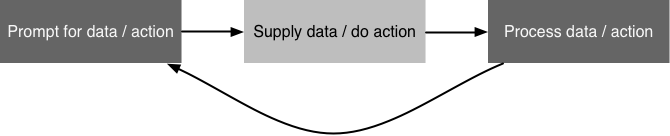
\includegraphics[width=\textwidth]{media/dialogue_sequence.png}
}

\frame{
    \frametitle{Gulfs in the dialogue}
    \begin{itemize}
        \item `Gaps' between control represent the \alert{Gulfs of E \& E}
        \item Gulf of Evaluation
        \begin{itemize}
            \item Understanding what the system is prompting for (or what the user needs to do)
        \end{itemize}
        \item Gulf of Execution
        \begin{itemize}
            \item Providing system with information or an action
        \end{itemize}
    \end{itemize}
}

\frame{
    \frametitle{System dialogue}
    \textbf{Main dialogue loop}
    \vskip20pt
    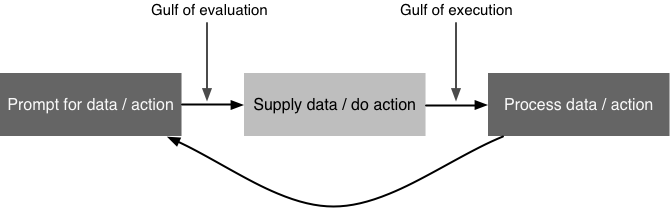
\includegraphics[width=\textwidth]{media/dialogue_sequence_2.png}
}

\frame{
    \frametitle{Considering system dialogue}
    \begin{itemize}
        \item In task analysis, we considered 
        \begin{itemize}
            \item Computer tasks
            \item Human tasks
            \item Combined tasks
        \end{itemize}
        \item Clear how these are represented as dialogue
    \end{itemize}
}

\frame{
    \frametitle{Considering system dialogue}
    \begin{itemize}
        \item When studying hardware interfaces, we considered
        \begin{itemize}
            \item Many different input devices
            \item Many different output devices
        \end{itemize}
        \item Dialogue style needs to consider type of I/O device
        \item Also, use in bridging Gulfs of E \& E
    \end{itemize}
}

\frame{
    \frametitle{Choosing suitable dialogues}
    \begin{itemize}
        \item Important to consider the main principles of HCI we've covered
        \item Use a sensible hardware interface
        \item Use a sensible software interface
        \item But also choose a sensible approach to dialogue!
        \begin{itemize}
            \item The `nicest looking' may not be the most usable
        \end{itemize}
    \end{itemize}
}

\frame{
    \frametitle{Comparing dialogues for tasks}
    \begin{itemize}
        \item Case: chess       
        \item Compare dialogue through:
        \begin{itemize}
            \item Command language
            \item Form
        \end{itemize}
    \end{itemize}
}

\frame{
    \frametitle{Comparing dialogues for tasks}
    \textbf{Firstly, what do users need to do?}
    \vskip20pt
    \begin{itemize}
        \item Identify tasks 
        \begin{itemize}
            \item Move to square (explicit)
            \item Take piece (explicit or implicit)
            \item Declare check (implicit)
            \item Declare checkmate (implicit)
        \end{itemize}
        \item Identify subtasks 
        \begin{itemize}
            \item Move to square \alert{square}
            \item Take piece at \alert{square}
        \end{itemize} 
    \end{itemize}
    \vskip10pt
    \textbf{The system needs to show the system state after each operation.}
}

\frame{
    \frametitle{Comparing dialogues for tasks}
    \textbf{Command languages}
    \begin{itemize}
        \item A very traditional dialogue style
        \item User agent issues a series of commands, system agent responds
        \item \alert{Arguments} are manually passed to commands
    \end{itemize}   
    \begin{center}
        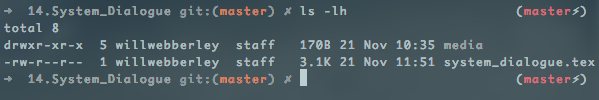
\includegraphics[width=\textwidth]{media/command.png}
    \end{center}
}

\frame{
    \frametitle{Comparing dialogues for tasks}
    \textbf{A command language for issuing \alert{chess} commands}
    \vskip20pt
    \alert{Human agent actions}
    \begin{itemize}
        \item Give commands, for example:
        \begin{itemize}
            \item \texttt{move -s D1 -d D2}
            \item \texttt{take -s C2 -d D4}
        \end{itemize}
    \end{itemize}
    \vskip20pt
    \alert{Computer agent actions}
    \begin{itemize}
        \item Show game state
        \item Prompt for user commands
        \item Display errors
        \begin{itemize}
            \item Missing pieces (e.g. already taken)
            \item Invalid move (e.g. sideways for a pawn)
        \end{itemize}
    \end{itemize}
}

\frame{
    \frametitle{Comparing dialogues for tasks}
    \textbf{Example of \alert{chess} moves using a \alert{command language}}
    \vskip20pt 
    \begin{columns}[t]
        \column{.25\textwidth}
            \alert{1: Computer}
            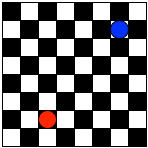
\includegraphics[width=\textwidth]{media/chess_1.png}
        \column{.25\textwidth}
            \alert{2: Human}\\
            \vskip15pt
            \footnotesize
            \texttt{move -s C2 -d D4}
        \column{.25\textwidth}
            \alert{3: Computer}
            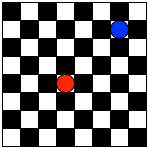
\includegraphics[width=\textwidth]{media/chess_2.png}
        \column{.25\textwidth} 
            \alert{4: Human}\\
            \vskip15pt
            \footnotesize
            \texttt{move -s D4 -d F5}
    \end{columns}
    \vskip10pt
    \begin{columns}[t]
        \column{.25\textwidth}
            \alert{5: Computer}
            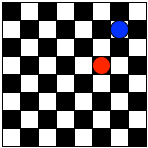
\includegraphics[width=\textwidth]{media/chess_3.png}
        \column{.25\textwidth}
            \alert{6: Human}\\
            \vskip15pt
            \footnotesize
            \texttt{take -s F5 -d G7}
        \column{.25\textwidth}
            \alert{7: Computer}
            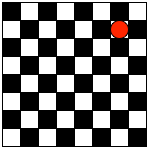
\includegraphics[width=\textwidth]{media/chess_4.png}
        \column{.25\textwidth} 
            \alert{8: Human}\\
            \vskip15pt
            \footnotesize
            \texttt{move -s G7 -d H5}
    \end{columns}
}   

\frame{
    \frametitle{Comparing dialogues for tasks}
    \begin{columns}[t]
        \column{.5\textwidth}
            \textbf{Command language advantages}
            \vskip10pt
            \begin{itemize}
                \item Very quick (only a few keyboard presses required)
                \item Not computationally intensive
                \item Usable on lower-fidelity displays
            \end{itemize}
        \column{.5\textwidth}
            \textbf{Command language disadvantages}
            \vskip10pt
            \begin{itemize}
                \item Cognitive burden (having to remember commands)
                \item Practice needed to master commands
                \item Little user control (e.g. how to exit? how to exit with saved game state?)
                \item Easy to make syntax errors
            \end{itemize}
    \end{columns}
}

\frame{
    \frametitle{Comparing dialogues for tasks}
    \textbf{Forms}
    \begin{itemize} 
        \item Information input for GUI systems
        \item Frequently used on the web
        \item \alert{Guided} information input
        \item System asks for exactly what it needs to know (with optional inputs)
    \end{itemize}   
    \begin{center}
        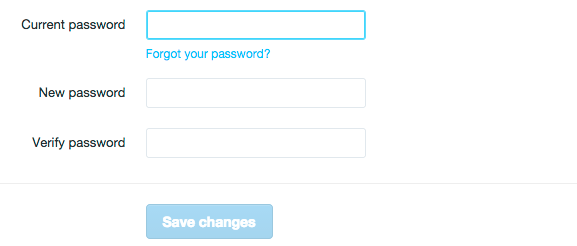
\includegraphics[width=.8\textwidth]{media/form_example.png}
    \end{center}
}

\frame{
    \frametitle{Comparing dialogues for tasks}
    \textbf{A form for issuing \alert{chess} commands}
    \vskip20pt
    \alert{Human agent actions}
    \begin{itemize}
        \item Complete a form, filling in all required info
        \item Submit the form for processing
    \end{itemize}
    \vskip20pt
    \alert{Computer agent actions}
    \begin{itemize}
        \item Show game state
        \item Display form
        \item Display errors
        \begin{itemize}
            \item Missing pieces (e.g. already taken)
            \item Invalid move (e.g. sideways for a pawn)
        \end{itemize}
    \end{itemize}
}

\frame{
    \frametitle{Comparing dialogues for tasks}
    \textbf{Example of \alert{chess} moves using a \alert{form}}
    \vskip20pt
    \begin{columns}[t]
        \column{.5\textwidth}
            \alert{1: Computer}
            \vskip10pt
            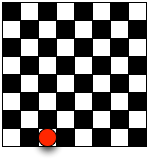
\includegraphics[width=\textwidth]{media/chess_5.png}
        \column{.5\textwidth}
            \alert{2: Human}
            \begin{center}
                \vskip10pt
                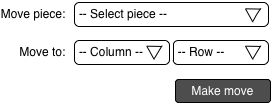
\includegraphics[width=.8\textwidth]{media/form_1.png}
                \vskip20pt
                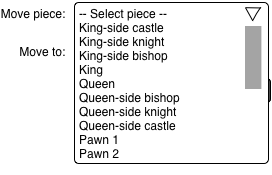
\includegraphics[width=.8\textwidth]{media/form_2.png}
            \end{center}
    \end{columns}    
}


\frame{
    \frametitle{Comparing dialogues for tasks}
    \textbf{Example of \alert{chess} moves using a \alert{form}}
    \vskip20pt
    \begin{columns}[t]
        \column{.5\textwidth}
            \alert{2: Human (cont'd)}
            \begin{center}
                \vskip10pt
                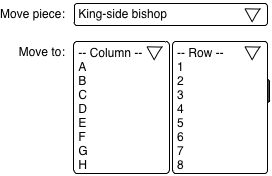
\includegraphics[width=.8\textwidth]{media/form_3.png}
                \vskip20pt
                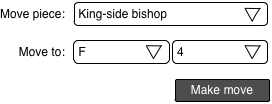
\includegraphics[width=.8\textwidth]{media/form_4.png}
            \end{center}
        \column{.5\textwidth}
            \alert{3: Computer}
            \vskip10pt
            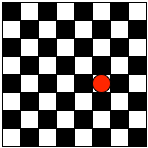
\includegraphics[width=\textwidth]{media/chess_6.png}
    \end{columns}    
}

\frame{
    \frametitle{Comparing dialogues for tasks}
    \begin{columns}[t]
        \column{.5\textwidth}
            \textbf{Form advantages}
            \vskip10pt
            \begin{itemize}
                \item Guided entry (e.g. impossible syntax errors)
                \item Better user control (easy to make buttons for saving/exiting)
                \item Richer game experience on higher fidelity displays
            \end{itemize}
        \column{.5\textwidth}
            \textbf{Form disadvantages}
            \vskip10pt
            \begin{itemize}
                \item Slow and clunky
                \item Not much \alert{flexibility} (even expert users have to complete all the fields)
            \end{itemize}
    \end{columns}
}

\frame{
    \frametitle{Comparing dialogues for tasks}
    \begin{itemize}
        \item Obviously, these are extreme examples
        \begin{itemize}
            \item Mobile apps would involve tapping/dragging
            \item Desktop/web apps would involve dragging mouse, etc.
        \end{itemize}
        \item But key is that different dialogues have advantages in different domains
        \item E.g. conversational interfaces (e.g. Siri, Google Now, SHERLOCK)
        \begin{itemize}
            \item Good for quick data entry that might be non-structured or complex
            \item But natural language not always fully understood by a machine agent
        \end{itemize}
    \end{itemize}
}

\frame{
    \frametitle{System states}
    \begin{itemize}
        \item Dialogues allow systems to change \alert{state}
        \item User input may cause system to assume different state
        \item System state may refer to, for example:
        \begin{itemize}
            \item Data held by system objects
            \item Constraint on available actions for user
            \item Constraint on system tasks
        \end{itemize}
        \item States can be mapped using \alert{state transition diagrams}
    \end{itemize}
}

\frame{
    \frametitle{State transition diagrams}
    \begin{itemize}
        \item These can capture dialogue
        \begin{itemize}
            \item As in task analysis (e.g. Jackson Structured Notation)
        \end{itemize}
        \item Also capture pathways and triggers between states:
        \begin{itemize}
            \item \alert{States} - discrete state of system
            \item \alert{Transitions} - triggers causing state change
            \item \alert{Paths} - allowed ordering (or sequencing) of states
        \end{itemize}
    \end{itemize}
    \vskip30pt
    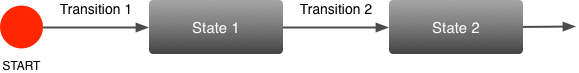
\includegraphics[width=\textwidth]{media/state_transition_diagram.png}
}

\frame{
    \frametitle{State transition diagrams}
    \textbf{Simple example for task: `Select bold'}
    \vskip30pt
    
\includegraphics[width=\textwidth]{media/state_transition_diagram_2.png}
}

\frame{
    \frametitle{State transition diagrams}
    \textbf{Simple example for task: `Style font'}
    \vskip30pt
    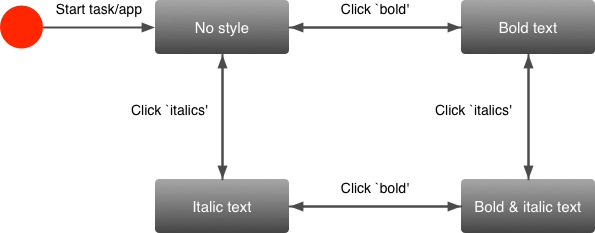
\includegraphics[width=\textwidth]{media/state_transition_diagram_3.png}
}

\frame{
    \frametitle{State transition diagrams}
    \textbf{Simple example for task: `Make phonecall'}
    \vskip30pt
    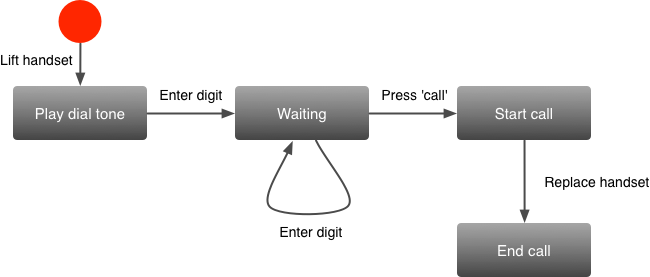
\includegraphics[width=\textwidth]{media/state_transition_diagram_4.png}
}

\frame{
    \frametitle{State transition diagrams}
    \begin{itemize}
        \item Should also model \alert{exit points}
        \begin{itemize}
            \item Which state to return to if `cancel' pressed?
        \end{itemize}
        \item System roles in dialogue usually given by \alert{states}
        \item User roles in dialogue usually given by \alert{transitions}
    \end{itemize}   
}

\frame{
    \frametitle{State transition diagrams}
    \textbf{These should consider...}
    \vskip10pt
    \begin{itemize}
        \item \alert{Completeness}
        \begin{itemize}
            \item Only some actions available in each state
            \item Designer should understand consequence of any action in a state
            \item Addresses \alert{Constraint}
        \end{itemize}
        \item \alert{Consistency}
        \begin{itemize}
            \item Expect same action in different states to do the same thing
            \item Addresses \alert{Familiarity} and \alert{Consistency}
        \end{itemize}
        \item \alert{Reachability}
        \begin{itemize}
            \item Ensure every state is reachable
            \item Ensure dialogue is fully connected
        \end{itemize}
        \item \alert{Reversability}
        \begin{itemize}
            \item Use arcs to allow backwards traversing
            \item Addresses \alert{User Control \& Freedom}
        \end{itemize}
    \end{itemize}
}

\frame{
     \frametitle{Revision questions}
     \begin{enumerate}
        \item What is `dialogue' in the context of interactive systems?
        \item What is meant by the term `agent' in system dialogue?
        \item Name three common types of dialogue.
        \item What is the relevance of the Gulf of E \& E in dialogue?
        \item What is a system state?
        \item Describe what the terms `path' and `transition' mean in the context of state transition diagrams.
     \end{enumerate}
}

\frame{
    \frametitle{Summary}
    \begin{itemize}
        \item System dialogue in interactive systems
        \item Human and computer agents
        \item Types and examples of system dialogue
        \item System states
        \item State transition diagrams
    \end{itemize}
}    

\end{document}
